\documentclass{beamer} % "Beamer" is a word used in Germany to mean video projector. 

\usetheme{Warsaw} % Search online for beamer themes to find your favorite or use the Berkeley theme as in this file.


\usecolortheme{spruce}


\usepackage{color} % It may be necessary to set PCTeX or whatever program you are using to output a .pdf instead of a .dvi file in order to see color on your screen.
\usepackage{graphicx} % This package is needed if you wish to include external image files.

\theoremstyle{definition} % See Lesson Three of the LaTeX Manual for more on this kind of "proclamation."
\newtheorem*{dfn}{A Reasonable Definition}               

\title{Quantitative Analysis of the effects of Kinesio Tape}
\author{Nathaniel Saul} 
\institute{University of Hawaii at Manoa}
%\date{January 6, 2012} 
% Remove the % from the previous line and change the date if you want a particular date to be displayed; otherwise, today's date is displayed by default.

\AtBeginSection[]  % The commands within the following {} will be executed at the start of each section.
{
\begin{frame} % Within each "frame" there will be one or more "slides."  
\frametitle{Presentation Outline} % This is the title of the outline.
\tableofcontents[currentsection]  % This will display the table of contents and highlight the current section.
\end{frame}
} % Do not include the preceding set of commands if you prefer not to have a recurring outline displayed during your presentation.

\begin{document}

\begin{frame} 
\titlepage
\end{frame}

\section{What is Kinesio Tape?} % Since this is the start of a new section, our recurring outline will appear here.

\begin{frame} 
\frametitle{Description of tape}


\begin{columns} % This creates a frame with multiple columns.

\begin{column}{0.5\textwidth} % Now begins our second column.
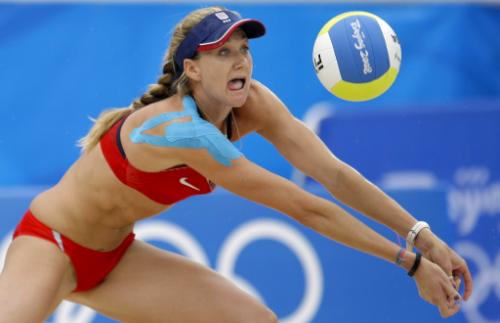
\includegraphics[width=5cm]{../images/kerri_walsh_kinesio.jpg} %

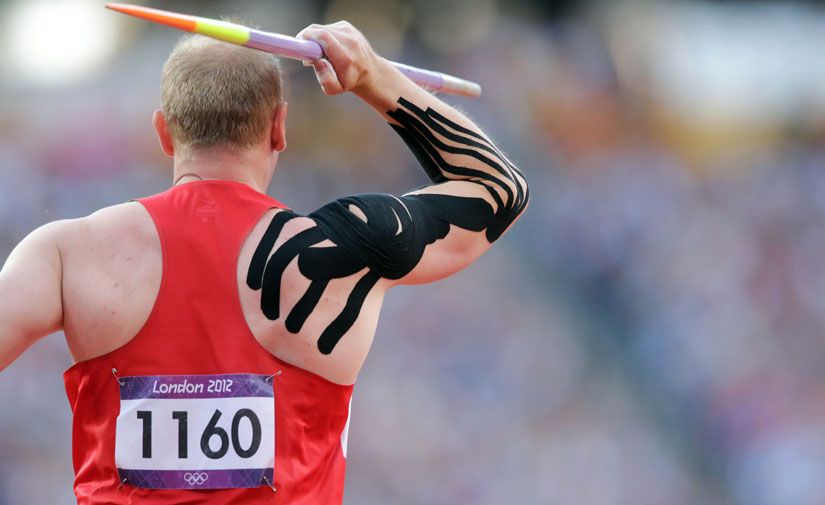
\includegraphics[width=5cm]{../images/olympic-javelin-kinesio-tape.jpg} 
\end{column}

\begin{column}{0.5\textwidth} % The first column will be 50% as wide as the width of text on the page.
\begin{itemize}
	\item Very stretchy tape applied to the skin
	\item Claimed benefits: \pause reduce pain, \pause prevent injury, \pause improve performance...
	\pause
	\item Allowed in professional sports.  
\end{itemize}
\end{column}


\end{columns}




\end{frame}



\begin{frame}
\frametitle{Hypothesis}


\begin{columns} % This creates a frame with multiple columns.

\begin{column}{0.5\textwidth} % Now begins our second column.
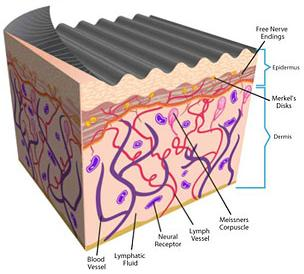
\includegraphics[width=5cm]{../images/k-tape-infographic.jpg} %

\end{column}

\begin{column}{0.5\textwidth} % The first column will be 50% as wide as the width of text on the page.
\begin{itemize}
\item expands region under skin
\item relieves pressure on nerves
\item allows for more blood flow
\end{itemize}
\end{column}


\end{columns}

\begin{center}
\pause 
{\Large This is only theory though - No objective studies! }
\end{center}
\end{frame}


\section{What do we do about it?} % Since this is the start of a new section, our recurring outline will appear here.

\begin{frame}
\frametitle{Use math!}

\begin{itemize}
\item Collect MRI images
\item Quantitatively analyze the region under the tape
\item Distill the change in shape to a simple yes or no.
\item Develop a general purpose method.
\end{itemize}
\end{frame}






%\begin{frame}
%\frametitle{Issues with data}
%very noisy... topological issues. handles make the data unusable to the algorithms - assume topologically equivalent to disk
%The region is then extracted.  They focus on the density to isolate the different regions, see F
%images of the not cleaned up thigh..  emphasis different connected components and the topological features.  
%- no central axis - each person is different size and laying differently through out.  
%\end{frame}


\section{What do we do with these images?}




\begin{frame}
\frametitle{Data}
\begin{columns} % This creates a frame with multiple columns.

\begin{column}{0.5\textwidth} % Now begins our second column.
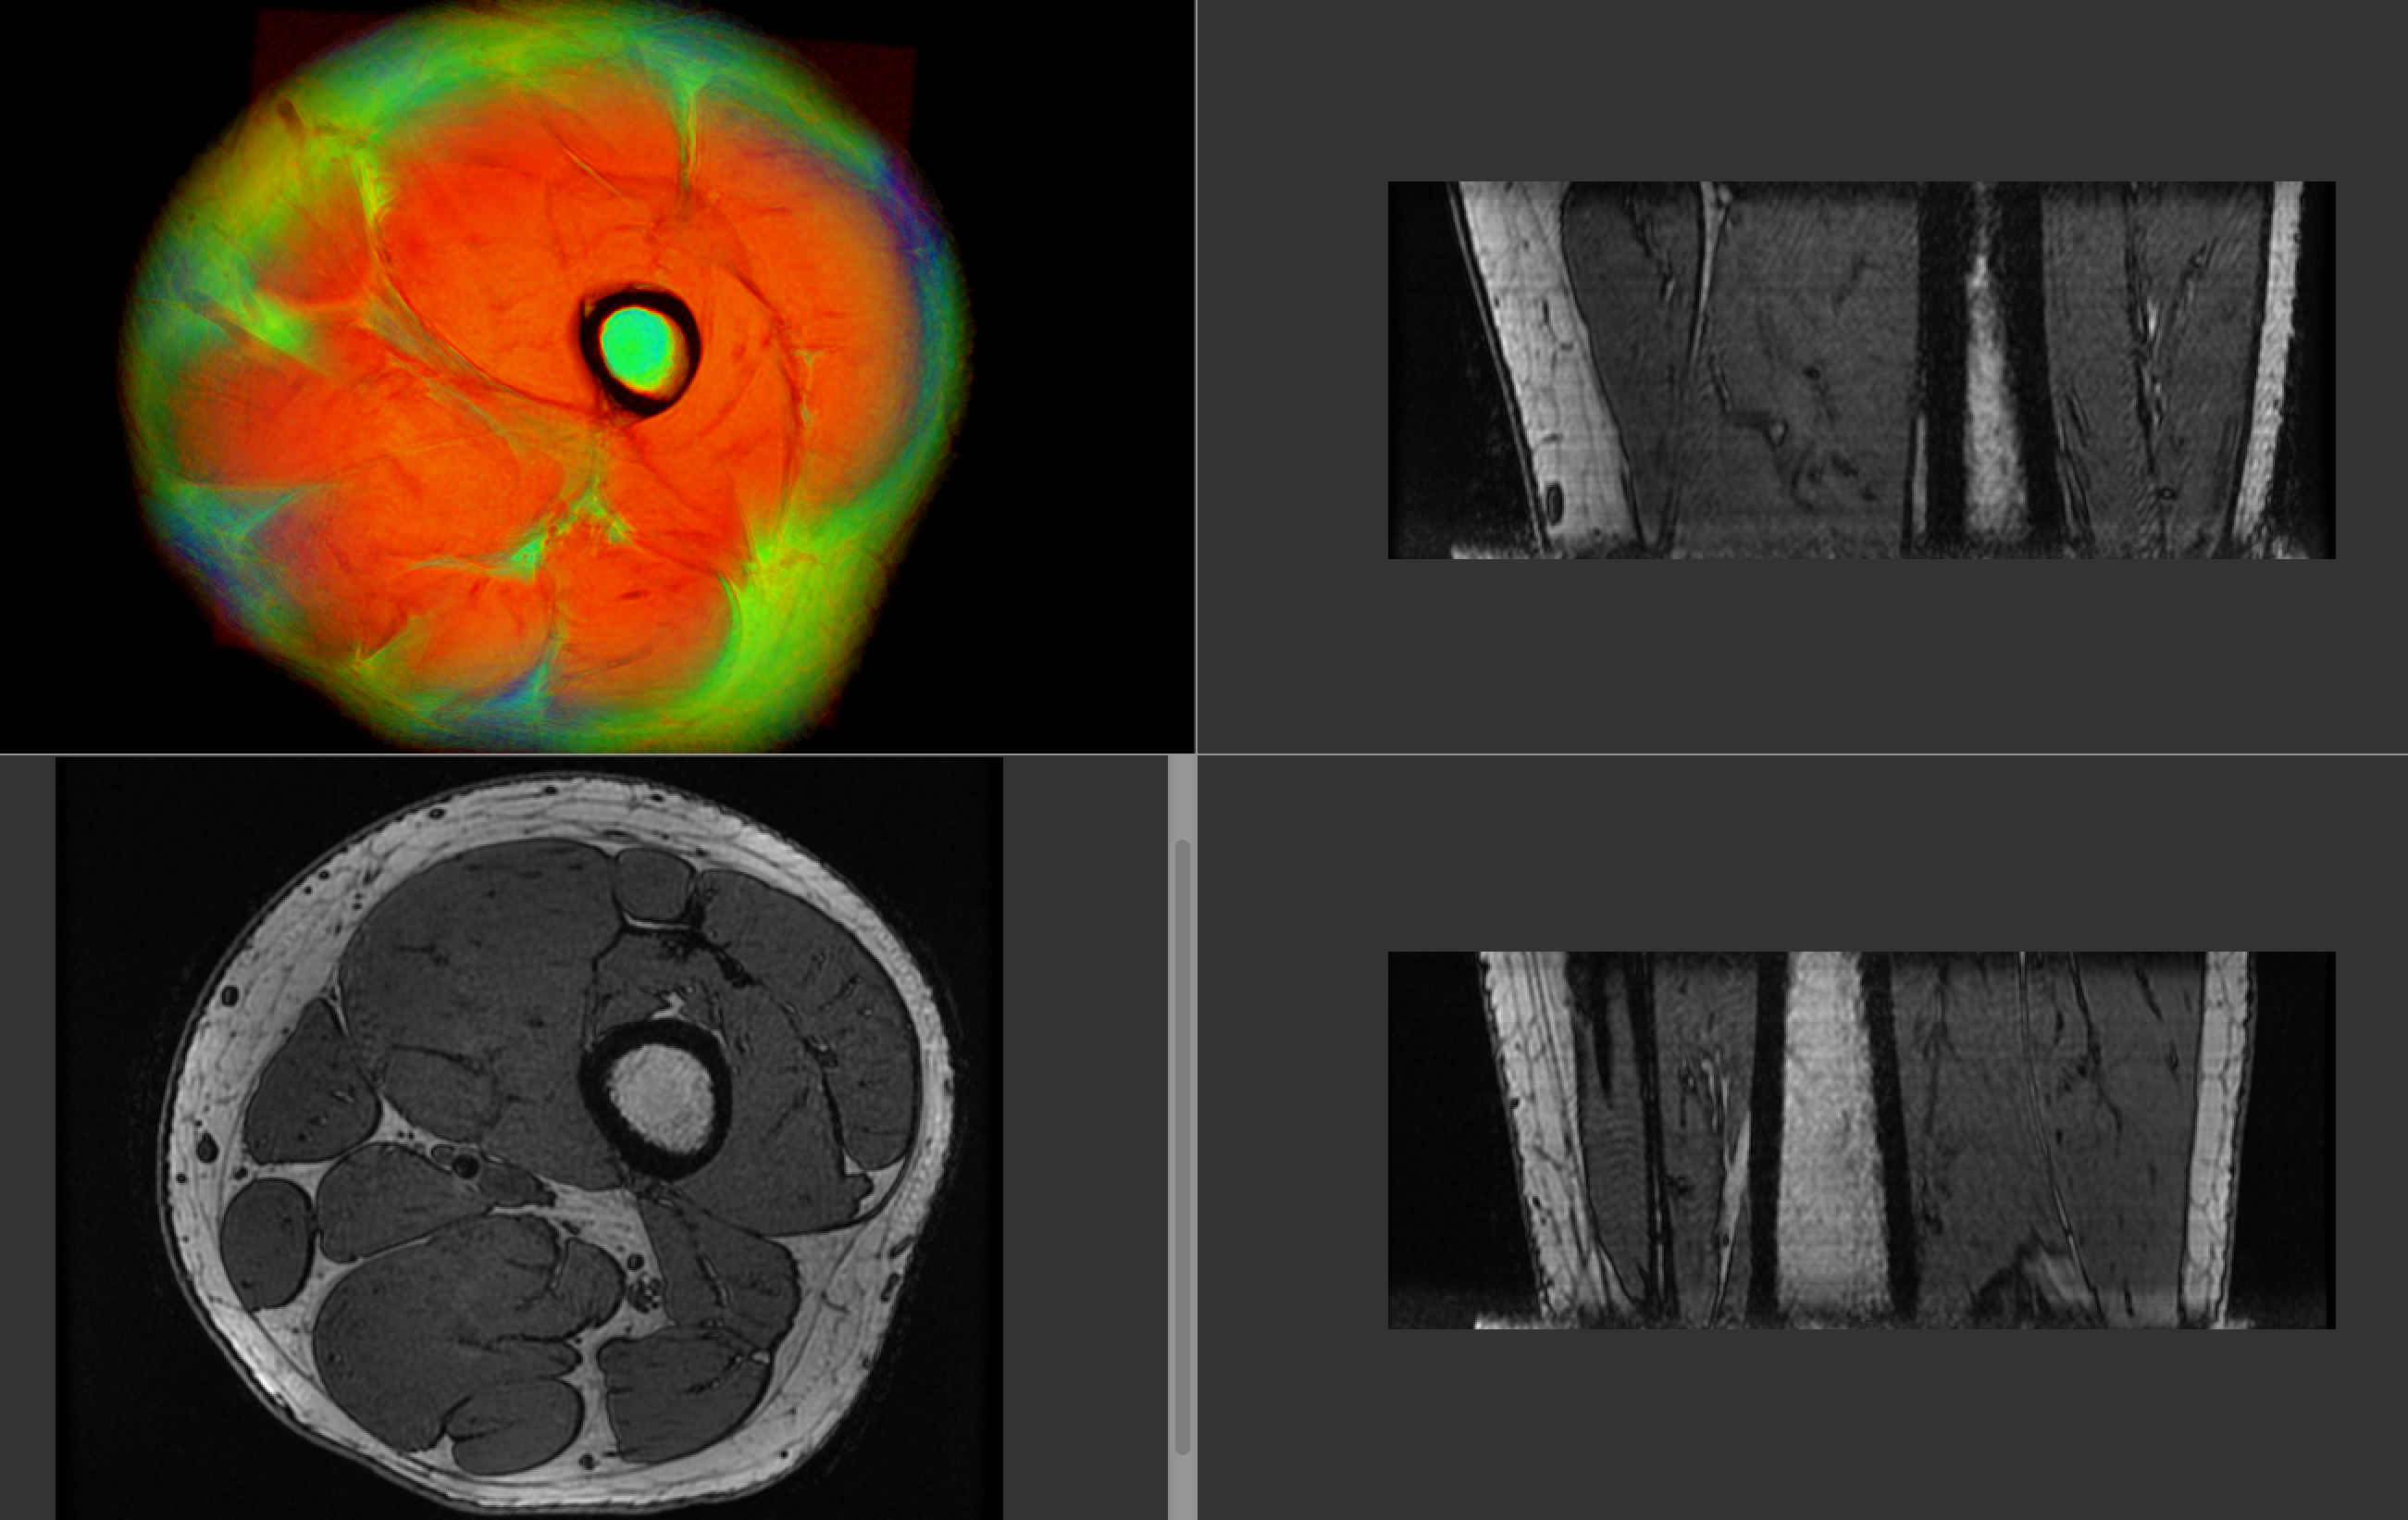
\includegraphics[width=5cm, height=5cm]{../images/thigh_colored.png}

\end{column}
\begin{column}{0.5\textwidth} % The first column will be 50% as wide as the width of text on the page.
\begin{itemize}
\item MRI of 40 patients
\item  ROI segmented based on density and oil drops
\item Triangulations

\end{itemize}
 
\end{column}

\end{columns}



\end{frame}

\begin{frame}
\frametitle{Region of Interest}
\begin{columns} % This creates a frame with multiple columns.

\begin{column}{0.5\textwidth} % Now begins our second column.
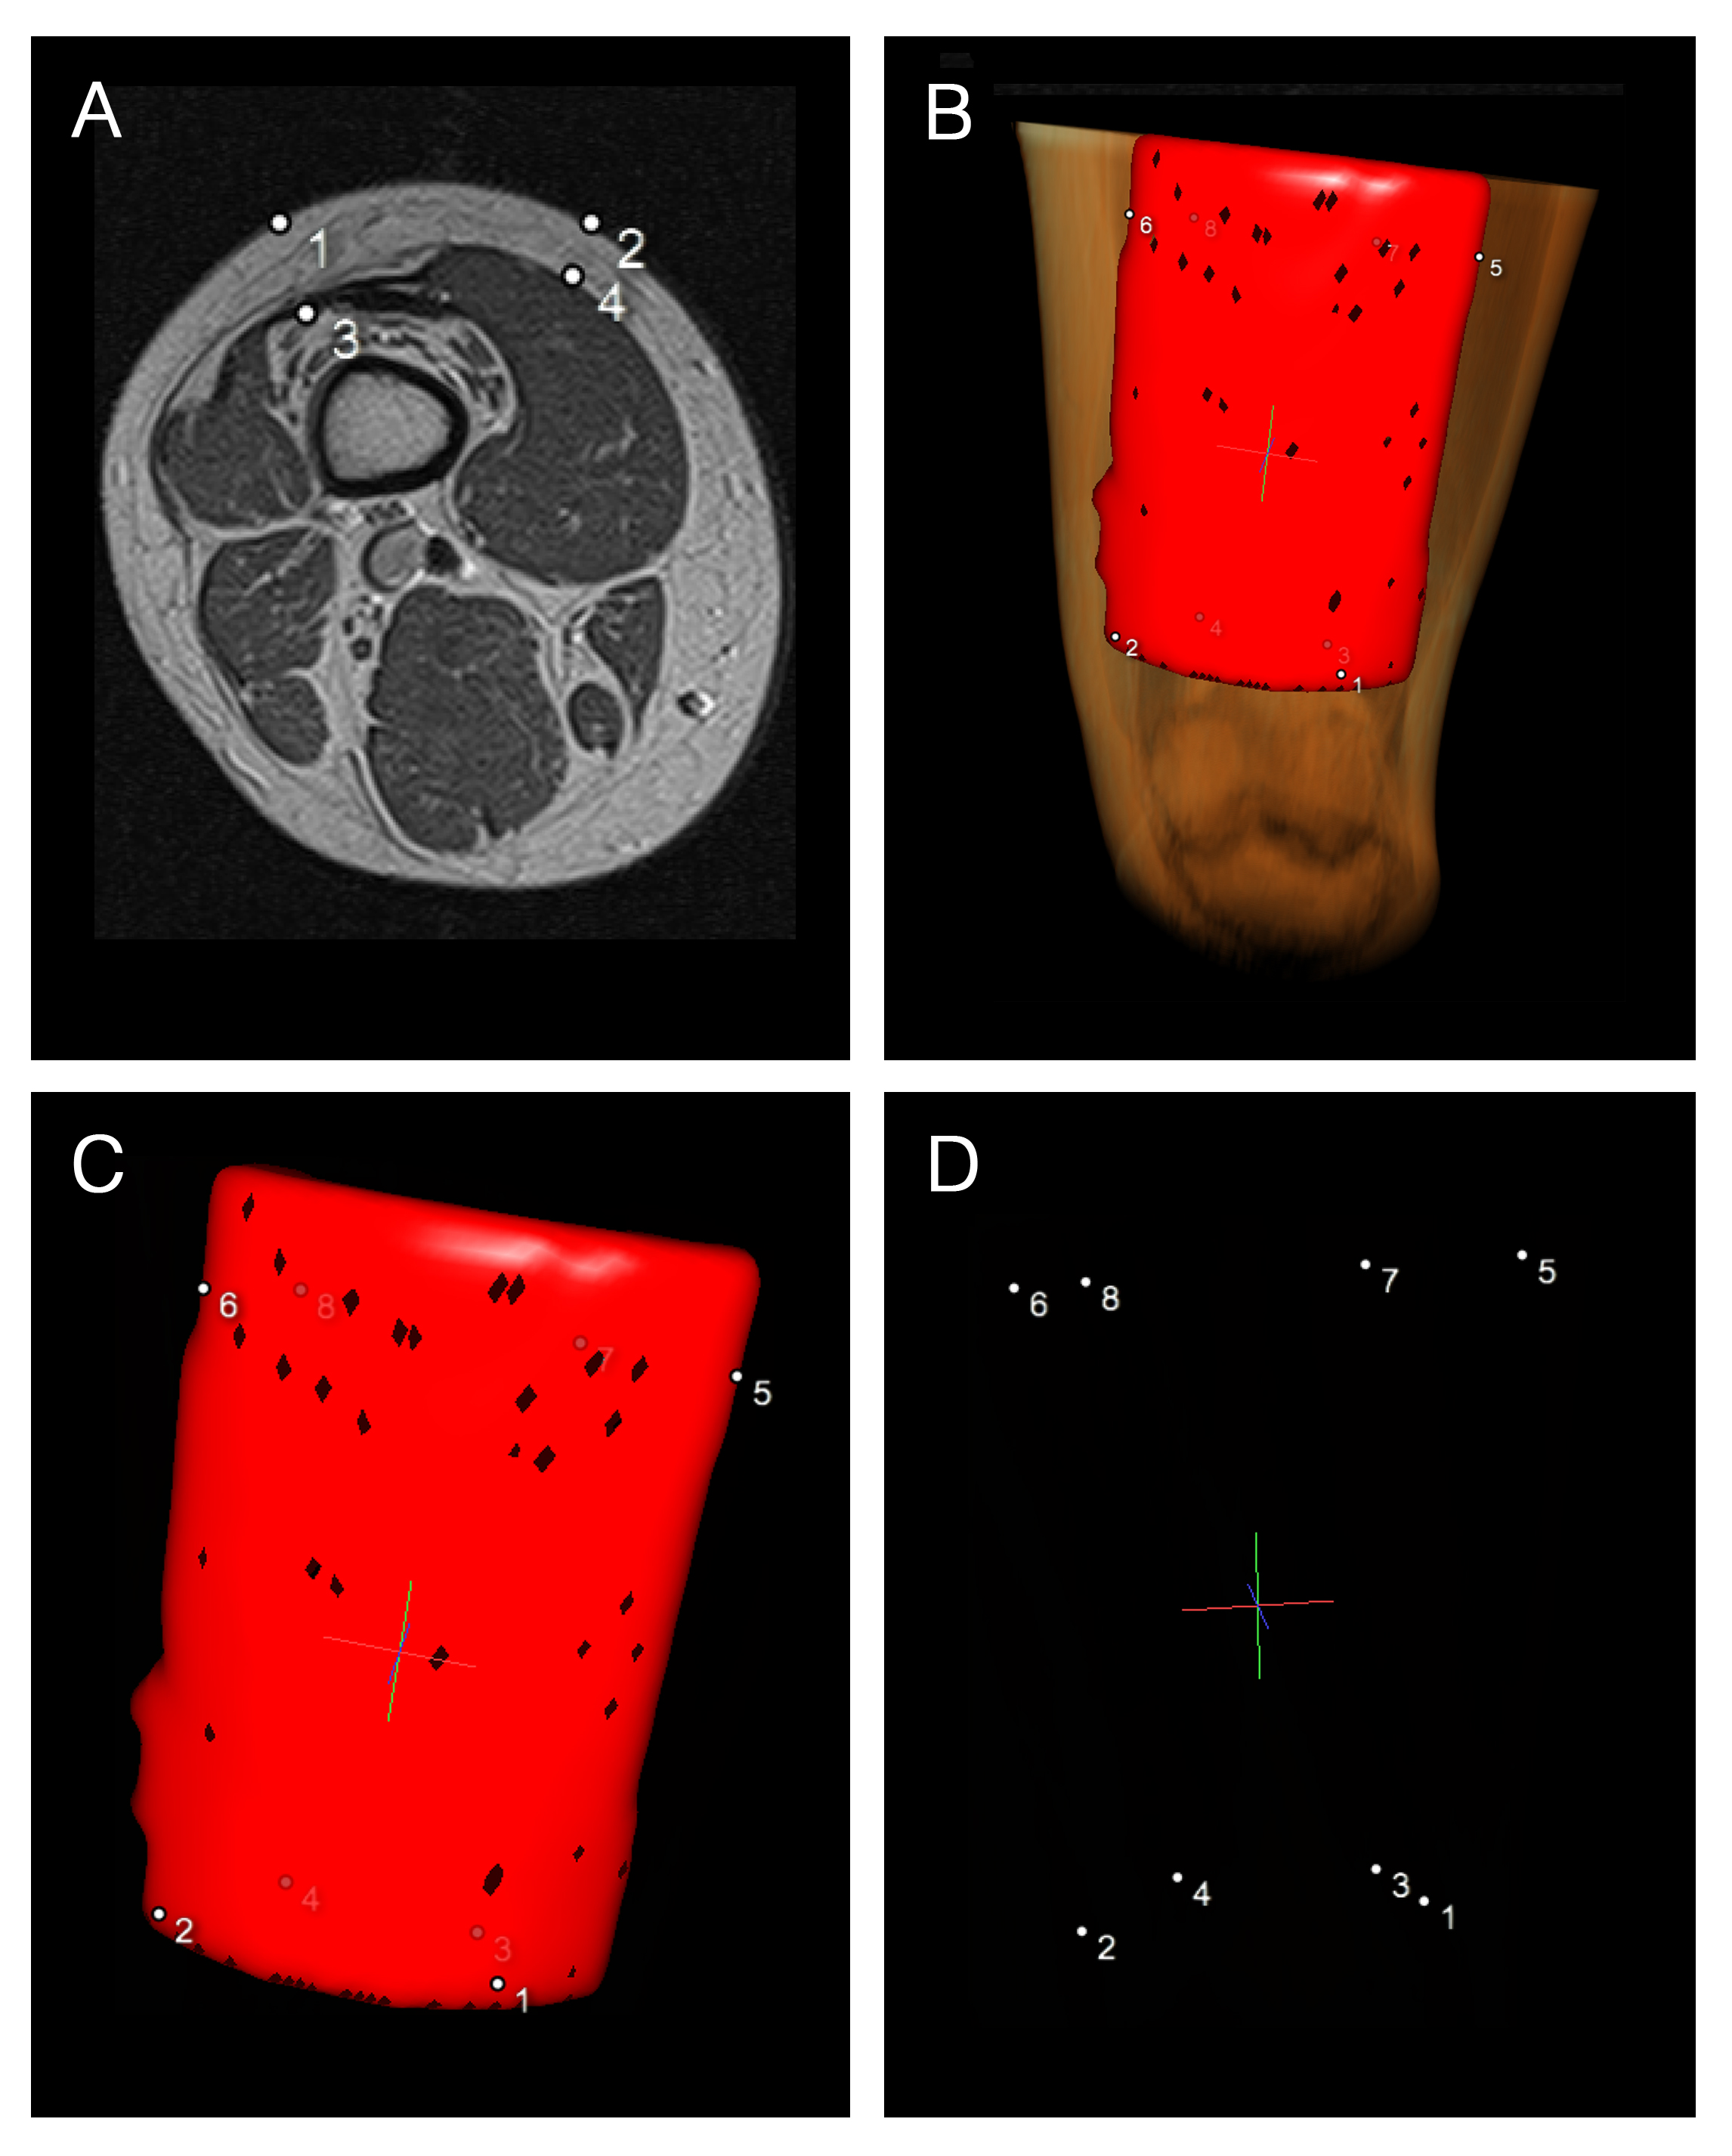
\includegraphics[width=5cm]{../images/thighwROI.jpg}

\end{column}
\begin{column}{0.5\textwidth} % The first column will be 50% as wide as the width of text on the page.
\begin{center}
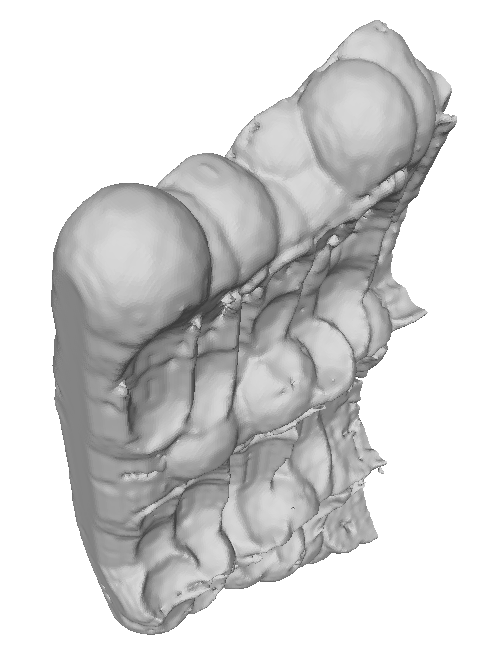
\includegraphics[height=3.5cm ]{../images/snapshot_angled02.png}

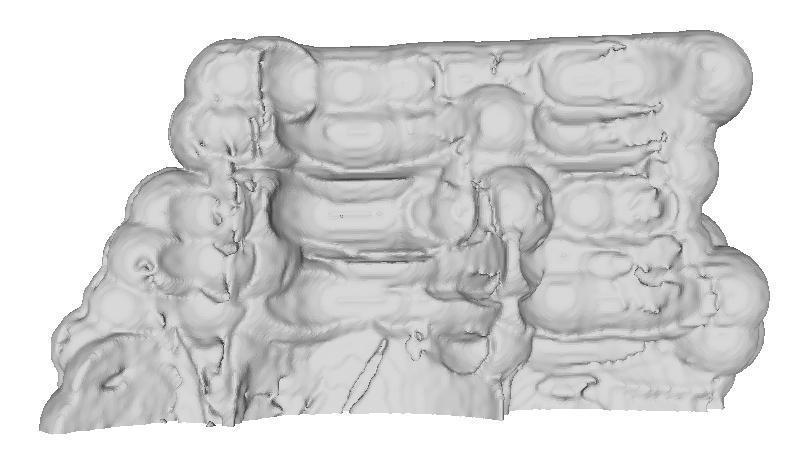
\includegraphics[height=2.5cm, ]{../images/snapshot_bottom00.png}
\end{center}
 
\end{column}

\end{columns}

\end{frame}


\begin{frame}
\frametitle{Clean and align}



\begin{columns} % This creates a frame with multiple columns.

\begin{column}{0.5\textwidth} % Now begins our second column.
\begin{itemize}
\item Use General Procrustes Method to align and resize all the shapes. 
\begin{itemize}
\item Affine transformations to align shapes as close as possible.
\end{itemize}
\item Remove separate components and topological impurities.
\end{itemize}
\end{column}
\begin{column}{0.5\textwidth} % The first column will be 50% as wide as the width of text on the page.
\begin{center}

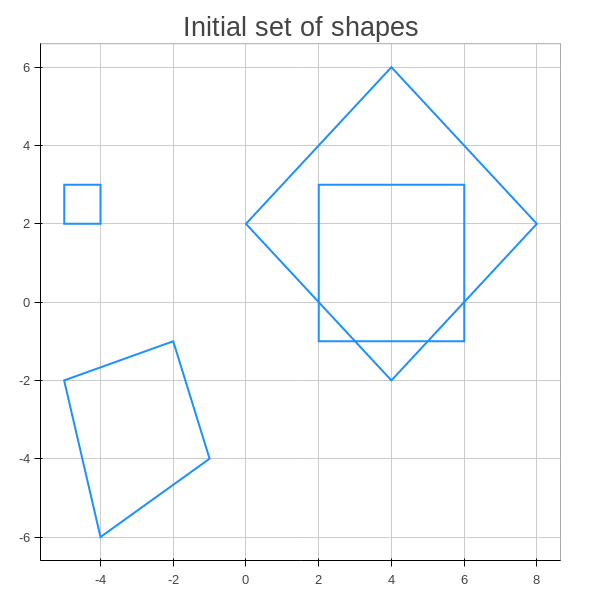
\includegraphics[width=3.5cm ]{../images/GPA_initial_shapes.png}

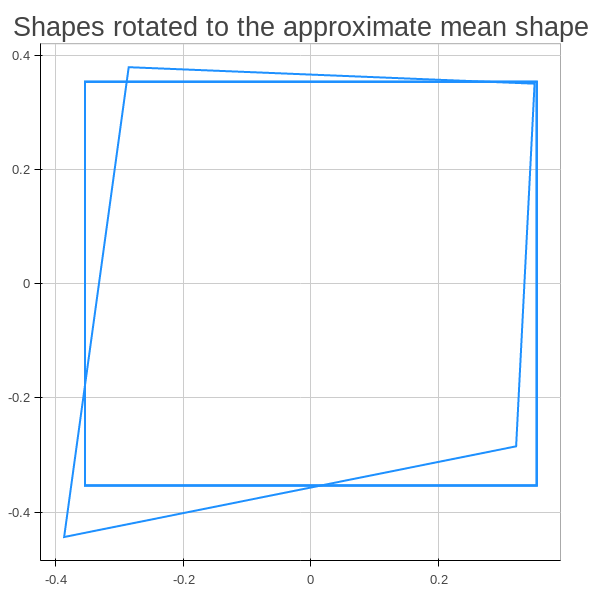
\includegraphics[width=3.5cm]{../images/GPA_rotated_shapes.png}
 
 \end{center}
\end{column}

\end{columns}

\end{frame}


\begin{frame}
\frametitle{Landmark based methods}

Look only at how the landmarks change between images.
\vspace{1cm}

\pause
\begin{itemize}
\item Hotelling's two sample t-test
\item Euclidean Distance Matrix Analysis

\end{itemize}




\end{frame}


\begin{frame}
\frametitle{Hotelling's two sample t-test. }

\begin{itemize}
\item multidimensional generalization of the t-test
\item compares the differences in positions of each point over time for each person.
\end{itemize}

$$ W = \frac{ \sum_{i=1}^{n_x} (x_i - \bar{x})( x_i - \bar{x})^T +  \sum_{i=1}^{n_y} (y_i - \bar{y})( y_i - \bar{y})^T}{ n_x + n_y - 2}$$

$$t^2 = \frac{n_x n_y}{n_x + n_y} (\bar{x} - \bar{y})^T W^{-1} (\bar{x} - \bar{y}) \sim T^2(p,n_x + n_y - 2)$$

\end{frame}

\begin{frame}
\frametitle{Euclidean Distance Matrix Analysis}

\begin{itemize}
\item Matrix encodes the distance between each shape
\item Difference between shape matrices can be calculated
\item Statistics can be done on these differences

\end{itemize}

\end{frame}

\begin{frame}
\frametitle{Entire ROI methods}
what if the corners don't change much? 



what if the shape wrinkles a little bit, but the corners stay constant?


\vspace{1cm}
\begin{columns}
\begin{column}{0.5\textwidth} % The first column will be 50% as wide as the width of text on the page.

\begin{center}
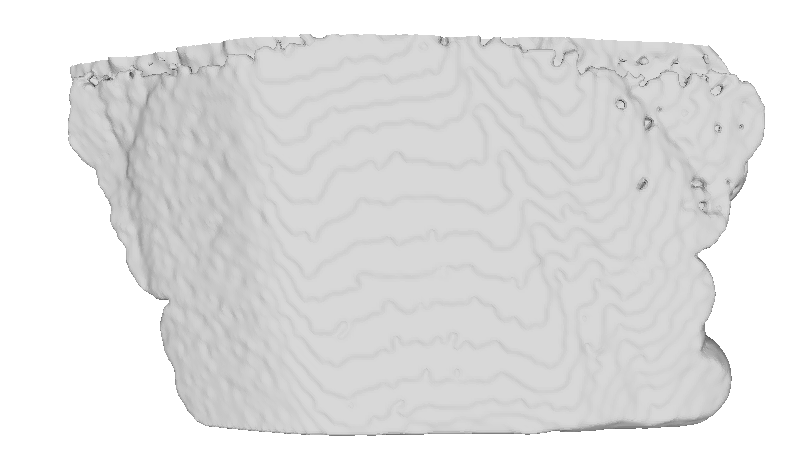
\includegraphics[width=3.5cm, ]{../images/snapshot_top01.png}
\end{center}

\end{column}


\begin{column}{0.5\textwidth} % The first column will be 50% as wide as the width of text on the page.

\begin{center}
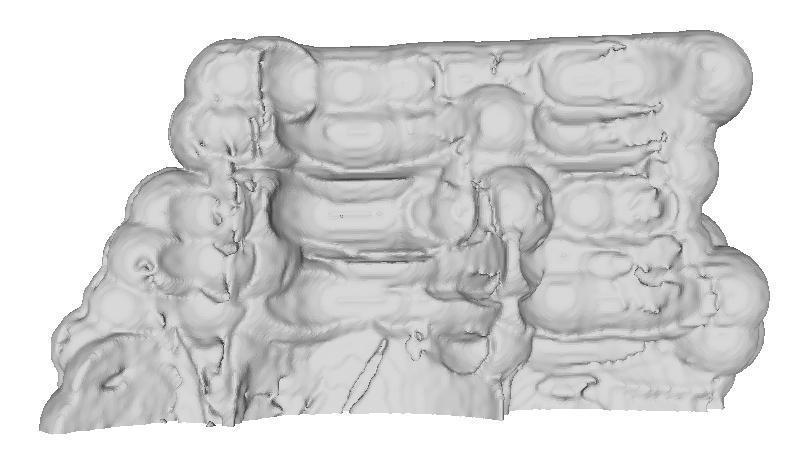
\includegraphics[width=3.5cm, ]{../images/snapshot_bottom00.png}
\end{center}

\end{column}


\end{columns}
\pause

\vspace{1cm}

800,000 vertices per shape and we're only looking at 8 of them!


\end{frame}


\begin{frame}
\frametitle{First step - parameterize the surface}
Standardizing all of the shapes by mapping each surface to the unit cube.


\begin{itemize}
\item 
 find the nearest neighboring vertex 
 \item
find the shortest paths between these vertices
\item 
 cut out the 6 sides of the shape
\item 
 map each side to the unit square 
\end{itemize}
\begin{center}
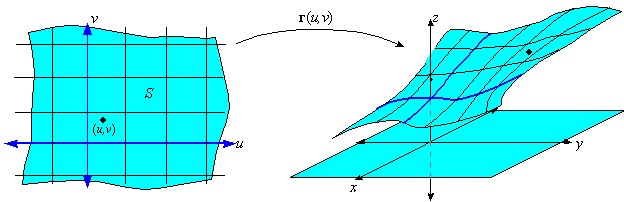
\includegraphics[height=2.5cm, ]{../images/param1b.jpg}
\end{center}
\end{frame}


\begin{frame}
\frametitle{Statistics on the parameterization}

\begin{itemize}

\item distances between the corresponding top and bottom points

\item map of p-values describing whether the change at that point across all the patients was significant  

\item persistence diagrams of parameterization map
\end{itemize}


\begin{columns}
\begin{column}{0.25\textwidth}
\begin{center}
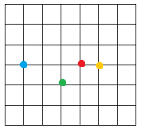
\includegraphics[height=2.5cm, ]{../images/unit_square.png}
\end{center}
\end{column}
\begin{column}{0.75\textwidth}

\begin{center}
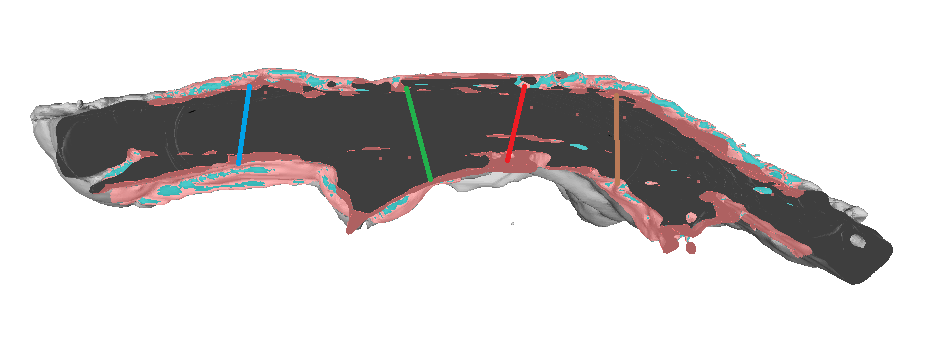
\includegraphics[height=2.5cm, ]{../images/cross_section00.png}
\end{center}
\end{column}

\end{columns}
\end{frame}


\begin{frame}

\frametitle{work is still continuing}
\begin{itemize}
\item waiting on the images
\item setting the corners of the parameterization.
\item computing persistence diagrams

\end{itemize}

\end{frame}


\begin{frame}
\frametitle{The End}
\begin{center}
Thank you
\end{center}
\end{frame}



\end{document}

